\documentclass[a4paper,11pt]{article} 
\usepackage{geometry}
\usepackage{circuitikz}
\usepackage[italian,english]{babel}
\geometry{
    a4paper,
    total={170mm,257mm},
    left=20mm,
    top=20mm,
}
\usepackage{graphicx}
\usepackage{caption}
\usepackage{subcaption}
\usepackage{multirow}
\usepackage{amsmath}
\captionsetup{tableposition=bottom,figureposition=bottom}
\captionsetup[figure]{labelfont=bf,textfont=it}
\captionsetup[table]{labelfont=bf,textfont=it}

\begin{document}
\title{Analisi della caratteristica tensione corrente in uscita di un BJT}
\author{Giovanni Bugli \and Giovanni Postacchini}
\date{Dicembre 2021, Postazione 15}

\maketitle
\begin{abstract}
  In questa esperienza di laboratorio è stata studiata la caratteristica tensione corrente in uscita per un transistor BJT pnp a emettitore comune. Il transtor è stato analizzato in regione attiva e sono stati stimati alcuni parametri caratteristici del transistor come la tensione di Early $V_{ey} = (20 \pm 3) V$, la conduttanza $g = (0.77 \pm 0.11) mS$ per una corrente di base $I_B \simeq -100 \mu A$ e $V_{ey} = (14 \pm 3) V$, $g = (1.7 \pm 0.3) mS$ per una corrente di base $I_B \simeq -200 \mu A$. Inoltre, è stato stimato il guadagno di corrente $\beta = (1.1 \pm 0.6) \cdot 10^2$.
\end{abstract}

\selectlanguage{italian}
\section{Introduzione}
Lo scopo di questa prova è quello di studiare il comportamento di un transistor BJT a emettitore comune analizzando i valori della corrente in funzione della tensione in uscita. In particolare è stata analizzata la regione  attiva in cui la caratteristica di uscita tensione-corrente del transistor ha un'andamento lineare del tipo:
\begin{equation}
  V = r \cdot I + V_{ey}
\end{equation}
dove i parametri sono rispettivamente $r$ la resistenza del BJT e $V_{ey}$ la tensione di Early. Dato r, è immediato ricavare la conduttanza g come $g = 1/r.$

Inoltre, è possibile stimare il guadagno di corrente $\beta$, per una certa tensione $V_{CE}$ fissata in regione attiva, secondo la formula:
\begin{equation}
  \beta = |\frac{\Delta I_C}{\Delta I_B}|
\end{equation}
dove $\Delta I_C$ è la differenza di corrente del collettore misurata per due valori di corrente di base distinti di differenza $\Delta I_B$.
\section{Apparato sperimentale e svolgimento}
\begin{figure}[h]
  \centering
  \begin{circuitikz}[american, scale = 1][europeanvoltages][smallR/.style={R, resistors/scale=0.7}]
    \draw
    (4 , 2)node[pnp, yscale = -1](pnp1){\ctikzflipy{BJT pnp}}
    (0,0) -- (0, 1) to[battery1, l = $-5 V$](0,2) -- (0, 3) -- (1, 3)
    (1, 2) -- (1,4)
    -- (2, 4) to[american potentiometer , l_ = $R_C  1 k \Omega$] (3,4) -- (4, 4)
    (1, 2) -- (2 ,2) to[american potentiometer, l_ = $R_B  100 k \Omega$] (3, 2) -- (pnp1.B)
    (4, 4) -- (pnp1.C)
    (pnp1.E) -- (4, 0) -- (0,0)
    (1, 0) node[ground, scale = 1.5]{}
    (pnp1.B) node[above]{B}
    (pnp1.E) node[right]{E}
    (pnp1.C) node[right]{C}

    ;
  \end{circuitikz}
  \caption{Schema del circuito realizzato per lo studio del transistor BJT pnp in configurazione ad emettitore comune.}
\end{figure}
Il circuito realizzato, come mostrato in Fig. 1, è formato dai seguenti componenti: un generatore di tensione costante da -5V riferito a massa, due potenziometri $R_C$ ed $R_B$ con fondoscala rispettivamente da 1$k\Omega$ e $100k\Omega$, il transistor pnp al silicio BJT 2N3906(BU). Per le misure di tensione si è utilizzato l'oscilloscopio analogico ISO-TECH modello ISR 622 mentre per quelle di corrente il multimetro digitale FLUKE modello 77 IV.

La risoluzione e la precisione specifiche del multimetro e dell'oscilloscopio relativi ai valori di fondo scala utilizzati nelle misure sono riportate in Tab 1. Le incertezze associate alle misure di tensione e corrente sono state calcolate come discusso in appendice.

\begin{table}[h!]
  \begin{center}
    \begin{tabular}{|c|c|c|c|}
      \hline
                                     & Fondo scala  & Risoluzione & Precisione           \\
      \hline
      Multimetro                     & $60.00 mA$   & $0.01 mA$   & 1.5\% + 2 digits     \\
      \hline
      \multirow{7}{*}{Oscilloscopio} & $10 mV/div$  & $1 mV$      & \multirow{7}{*}{3\%} \\
                                     & $20 mV/div$  & $2 mV$      &                      \\
                                     & $50 mV/div$  & $5 mV$      &                      \\
                                     & $100 mV/div$ & $10 mV$     &                      \\
                                     & $200 mV/div$ & $20 mV$     &                      \\
                                     & $500 mV/div$ & $50 mV$     &                      \\
                                     & $1 V/div$    & $100 mV$    &                      \\
      \hline
    \end{tabular}
    \caption{Risoluzione e precisione degli strumenti di misura nei fondo scala utilizzati. La risoluzione dell'oscilloscopio è stata calcolata come fondoscala/10.}
  \end{center}
\end{table}

I componenti sono stati montati su una scheda millepori alla quale sono stati collegati opportunamente anche il generatore di tensione e gli strumenti di misura quali il multimetro e l'oscilloscopio. In particolare, per misurare la corrente $I_C$ si è collegato il multimetro in serie presso il collettore e per misurare la tensione $V_{CE}$ è stata collegata la sonda del multimetro, riferito a massa, sempre presso il collettore (punto C Fig. 1).
Per studiare la caratteristica di uscita tensione-corrente del transistor si è fissato il valore della corrente $I_B$ in corrispondenza della base B e si è proceduto a misurare la corrente del collettore $I_C$ variando tramite il potenziometro $R_C$ la tensione $V_{CE}$.
\newline
In un primo momento si è fissato il potenziometro $R_B$ in modo tale da avere $I_B \simeq -100 \mu A$,  ed in un secondo momento si è impostato $I_B \simeq -200 \mu A$. Le misure d $I_C$ e $V_{CE}$ sono state effetuate in un range di tensioni per $V_{CE}$ da -0.05 V a -4 V circa.

\section{Risultati e discussione}

I dati sperimentali relativi alla tensione e alla corrente nel piano di uscita misurati sono riportati in Tab. 2 e Tab. 3 in appendice B.
Siccome viene studiato un transistor pnp, i valori di tensione e corrente sono negativi, perciò per graficare i punti sperimentali sono stati constiderati i valori assoluti.

In Fig 3 sono graficati i punti sperimentali acquisiti per una corrente di base $I_B = -(0.10 \pm 0.02) mA$ e $ I_B = - (0.10 \pm 0.02) mA$.
In regione attiva, sono ben visibili i due diversi valori di corrente del collettore e le due diverse pendenze delle rette. In particolare, per $I_B \simeq -200 \mu A$ si osserva, a parità di tensione $V_{CE}$, una corrente del collettore maggiore in valore assoluto che per $I_B \simeq - 100 \mu A$, compatibile a quanto atteso.

Sui dati di tensione e corrente è stato eseguito un fit con l'Eq. 1 in un range di tensioni $V_{CE}$ da -1.4V a -4V, cioè dove la dipendenza tensione-corrente è in buona approssimazione lineare. In Fig. 4 vengono rappresentate le curve caratteristiche.
Dai parametri del fit lineare si ricavano dunque la tensione di Early e la resistenza: $V_{ey} = (20 \pm 3) V$, $r = (1.29 \pm 0.18) k\Omega$ con corrente di base  $I_B \simeq -100 \mu A$ ; $V_{ey} = (14 \pm 3) V$, $r = (0.59 \pm 0.09) k\Omega$ con corrente di base $I_B \simeq -200 \mu A$.
Dalla stima di r è possibile ricavare la conduttanza g come $g = 1/r$, con incertezza propagata $\Delta g = \Delta r/ r^2$. Per cui si ottiene: $g = (0.77 \pm 0.11) mS$ con $I_B \simeq -100 \mu A$, $g = (1.7 \pm 0.3)mS$ con $I_B \simeq -200 \mu A$.
Infine, scelto $V_{CE} = -3.1 V$, viene valutata la differenza dei valori delle correnti del collettore $I_C$ per le due curve, e si ottiene una stima del guadagno di corrente tramite l'Eq. 2  : $\beta =(1.1 \pm 0.6) \cdot 10^2$. L'incertezza associata al guadagno di corrente è stata calcolata come mostrato in appendice A. Si nota un grande errore relativo del guadagno di corrente che è legato all'incertezza associata alle misure delle correnti di base che è assai elevata.

\begin{figure}[h!]
  \centering
  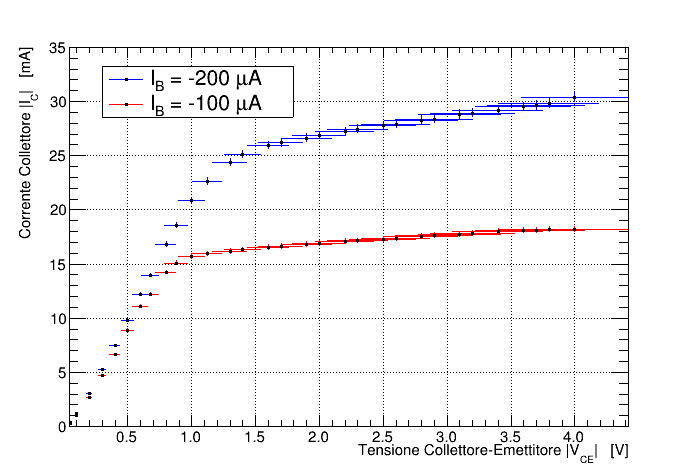
\includegraphics[width = 0.7\linewidth]{../analisi_dati/IVdati.png}
  \caption{Curve caratteristiche di tensione e corrente in uscita misurate con due diverse correnti di base $I_B$ come riportato in legenda. }
\end{figure}

\begin{figure} [h]
  \begin{subfigure}{0.49\textwidth}
    \centering
    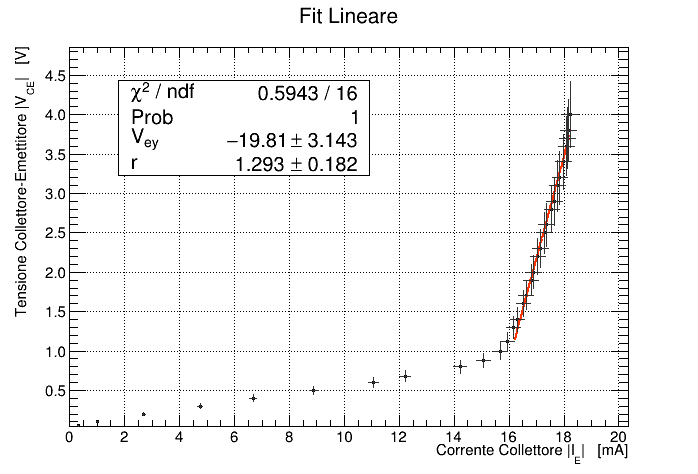
\includegraphics[width = \textwidth]{../analisi_dati/IV100_inverted.png}
    \subcaption{Caratteristica per $I_B \simeq -100 \mu A$}
  \end{subfigure}
  \begin{subfigure}{0.49\textwidth}
    \centering
    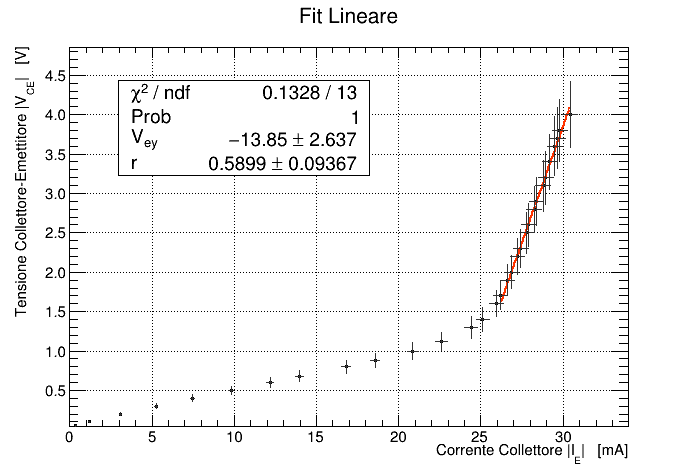
\includegraphics[width = \textwidth]{../analisi_dati/IV200_inverted.png}
    \subcaption{Caratteristica per $I_B \simeq -200 \mu A$}
  \end{subfigure}
  \caption{Caratteristica tensione-corrente in uscita del transistor sotto due distinte correnti di base $I_B$. La linea rossa rappresenta il fit lineare eseguito sui punti sperimentali in un range di tensioni  1.4 - 4 V. I parametri stimati dal fit sono riportati in legenda.}
\end{figure}

\clearpage
\section{Conclusioni}
L'esperimento ha confermato l'andamento atteso per la caratteristica del BJT in regione attiva. Sono stati ricavati i parametri dal fit corrispondenti alla tensione di Early e alla conduttanza, numericamente $V_{ey} = (20 \pm 3) V$, $g = (0.77 \pm 0.11) mS$ per una corrente di base  $I_B = - (0.10 \pm 0.02) mA$ e $V_{ey} = (14 \pm 3) V$, $g = (1.7 \pm 0.3)mS$ per una corrente di base $I_B = -(0.20 \pm 0.02) mA$. Il guadagno di corrente stimato è $\beta =(1.1 \pm 0.6) \cdot 10^2$.

\appendix
\section{Stima delle Incetezze}
L'incertezza sulle misure di corrente effettuate con il multimetro è 1.25\% della lettura + 2 digits. L'incertezza sulle misure di tensione effettuate con l'oscilloscopio $\sigma_{osc}$ è stata calcolata sommando in quadratura l'errore sulla lettura $\sigma_L$, l'errore sullo zero $\sigma_Z$ e l'errore del costruttore $\sigma_C$ secondo la formula:
\begin{equation*}
  \sigma_{osc} = \sqrt{\sigma_{L}^2+ \sigma_{Z}^2+ \sigma_{C}^2}
\end{equation*}
dove l'errore sulla lettura è $fondo scala / 10$ mentre $\sigma_{C}$ corrisponde al 3\% della lettura.

Per determinare l'incertezza sul guadagno di corrente possiamo riscrivere $\beta$ in funzione delle correnti misurate direttamente:
\begin{equation*}
  \beta = |\frac{I_{C2} - I_{C1}}{I_{B2} - I_{B1}}|
\end{equation*}
Siccome ciascuna misura di corrente ha un'incertezza associata $\Delta I$, l'incertezza del guadagno di corrente risulta essere:
\begin{equation*}
  \Delta\beta = \frac{\Delta I_{C1} + \Delta I_{C2}}{|I_{B2} - I_{B1}|} + \frac{|I_{C2} - I_{C1}|}{(I_{B2}- I_{B1})^2} (\Delta I_{B1} + \Delta I_{B2})
\end{equation*}

\newpage
\section{Dati Sperimentali}
\begin{table}[h!]
  \begin{center}
    \begin{tabular}{c|c|c|c}
      \textbf{$V_{CE}$ (V)} & \textbf{Fscala (V/div)} & \textbf{$I_{C}$ (mA)} & \textbf{Fscala (mA)} \\
      \hline
      $ -0.050 \pm 0.005 $  & 0.01                    & $ -0.310 \pm 0.015 $  & 60.00                \\
      $ -0.100 \pm 0.010 $  & 0.02                    & $ -1.00 \pm 0.03 $    & 60.00                \\
      $ -0.20 \pm 0.02 $    & 0.05                    & $ -2.69 \pm 0.05 $    & 60.00                \\
      $ -0.30 \pm 0.03 $    & 0.05                    & $ -4.75 \pm 0.08 $    & 60.00                \\
      $ -0.40 \pm 0.04 $    & 0.10                    & $ -6.68 \pm 0.11 $    & 60.00                \\
      $ -0.50 \pm 0.05 $    & 0.10                    & $ -8.89 \pm 0.14 $    & 60.00                \\
      $ -0.60 \pm 0.06 $    & 0.10                    & $ -11.05 \pm 0.18 $   & 60.00                \\
      $ -0.68 \pm 0.07 $    & 0.20                    & $ -12.22 \pm 0.19 $   & 60.00                \\
      $ -0.80 \pm 0.08 $    & 0.20                    & $ -14.2 \pm 0.2 $     & 60.00                \\
      $ -0.88 \pm 0.09 $    & 0.20                    & $ -15.1 \pm 0.2 $     & 60.00                \\
      $ -1.00 \pm 0.10 $    & 0.20                    & $ -15.7 \pm 0.2 $     & 60.00                \\
      $ -1.12 \pm 0.12 $    & 0.20                    & $ -15.9 \pm 0.2 $     & 60.00                \\
      $ -1.30 \pm 0.14 $    & 0.50                    & $ -16.2 \pm 0.3 $     & 60.00                \\
      $ -1.40 \pm 0.15 $    & 0.50                    & $ -16.3 \pm 0.3 $     & 60.00                \\
      $ -1.60 \pm 0.17 $    & 0.50                    & $ -16.5 \pm 0.3 $     & 60.00                \\
      $ -1.70 \pm 0.18 $    & 0.50                    & $ -16.6 \pm 0.3 $     & 60.00                \\
      $ -1.90 \pm 0.20 $    & 0.50                    & $ -16.8 \pm 0.3 $     & 60.00                \\
      $ -2.0 \pm 0.2 $      & 0.50                    & $ -16.9 \pm 0.3 $     & 60.00                \\
      $ -2.2 \pm 0.2 $      & 0.50                    & $ -17.1 \pm 0.3 $     & 60.00                \\
      $ -2.3 \pm 0.2 $      & 0.50                    & $ -17.1 \pm 0.3 $     & 60.00                \\
      $ -2.5 \pm 0.3 $      & 0.50                    & $ -17.3 \pm 0.3 $     & 60.00                \\
      $ -2.6 \pm 0.3 $      & 0.50                    & $ -17.4 \pm 0.3 $     & 60.00                \\
      $ -2.8 \pm 0.3 $      & 0.50                    & $ -17.6 \pm 0.3 $     & 60.00                \\
      $ -2.9 \pm 0.3 $      & 0.50                    & $ -17.7 \pm 0.3 $     & 60.00                \\
      $ -3.1 \pm 0.3 $      & 1.00                    & $ -17.8 \pm 0.3 $     & 60.00                \\
      $ -3.2 \pm 0.3 $      & 1.00                    & $ -17.9 \pm 0.3 $     & 60.00                \\
      $ -3.4 \pm 0.4 $      & 1.00                    & $ -18.0 \pm 0.3 $     & 60.00                \\
      $ -3.6 \pm 0.4 $      & 1.00                    & $ -18.1 \pm 0.3 $     & 60.00                \\
      $ -3.7 \pm 0.4 $      & 1.00                    & $ -18.1 \pm 0.3 $     & 60.00                \\
      $ -3.8 \pm 0.4 $      & 1.00                    & $ -18.2 \pm 0.3 $     & 60.00                \\
      $ -4.0 \pm 0.4 $      & 1.00                    & $ -18.2 \pm 0.3 $     & 60.00                \\
    \end{tabular}
    \caption{Dati sperimentali di tensione collettore-emettitore e corrente del collettore con corrente della base fissa $I_B \simeq -100 \mu A$. Per ogni misura viene riportata l'incertezza e il fondo scala utilizzato in fase di misurazine }
  \end{center}
\end{table}

\begin{table}[h!]
  \begin{center}
    \begin{tabular}{c|c|c|c}
      \textbf{$V_{CE}$ (V)} & \textbf{Fscala (V/div)} & \textbf{$I_{C}$ (mA)} & \textbf{Fscala (mA)} \\
      \hline
      $ -0.050 \pm 0.005 $  & 0.01                    & $ -0.370 \pm 0.016 $  & 60.00                \\
      $ -0.100 \pm 0.010 $  & 0.02                    & $ -1.19 \pm 0.03 $    & 60.00                \\
      $ -0.20 \pm 0.02 $    & 0.05                    & $ -3.09 \pm 0.06 $    & 60.00                \\
      $ -0.30 \pm 0.03 $    & 0.05                    & $ -5.25 \pm 0.09 $    & 60.00                \\
      $ -0.40 \pm 0.04 $    & 0.10                    & $ -7.45 \pm 0.12 $    & 60.00                \\
      $ -0.50 \pm 0.05 $    & 0.10                    & $ -9.81 \pm 0.16 $    & 60.00                \\
      $ -0.60 \pm 0.06 $    & 0.10                    & $ -12.19 \pm 0.19 $   & 60.00                \\
      $ -0.68 \pm 0.07 $    & 0.20                    & $ -13.9 \pm 0.2 $     & 60.00                \\
      $ -0.80 \pm 0.08 $    & 0.20                    & $ -16.8 \pm 0.3 $     & 60.00                \\
      $ -0.88 \pm 0.09 $    & 0.20                    & $ -18.6 \pm 0.3 $     & 60.00                \\
      $ -1.00 \pm 0.10 $    & 0.20                    & $ -20.9 \pm 0.3 $     & 60.00                \\
      $ -1.12 \pm 0.12 $    & 0.20                    & $ -22.6 \pm 0.3 $     & 60.00                \\
      $ -1.30 \pm 0.14 $    & 0.50                    & $ -24.4 \pm 0.4 $     & 60.00                \\
      $ -1.40 \pm 0.15 $    & 0.50                    & $ -25.1 \pm 0.4 $     & 60.00                \\
      $ -1.60 \pm 0.17 $    & 0.50                    & $ -25.9 \pm 0.4 $     & 60.00                \\
      $ -1.70 \pm 0.18 $    & 0.50                    & $ -26.2 \pm 0.4 $     & 60.00                \\
      $ -1.90 \pm 0.20 $    & 0.50                    & $ -26.6 \pm 0.4 $     & 60.00                \\
      $ -2.0 \pm 0.2 $      & 0.50                    & $ -26.9 \pm 0.4 $     & 60.00                \\
      $ -2.2 \pm 0.2 $      & 0.50                    & $ -27.2 \pm 0.4 $     & 60.00                \\
      $ -2.3 \pm 0.2 $      & 0.50                    & $ -27.4 \pm 0.4 $     & 60.00                \\
      $ -2.5 \pm 0.3 $      & 0.50                    & $ -27.8 \pm 0.4 $     & 60.00                \\
      $ -2.6 \pm 0.3 $      & 0.50                    & $ -27.9 \pm 0.4 $     & 60.00                \\
      $ -2.8 \pm 0.3 $      & 0.50                    & $ -28.2 \pm 0.4 $     & 60.00                \\
      $ -2.9 \pm 0.3 $      & 0.50                    & $ -28.4 \pm 0.4 $     & 60.00                \\
      $ -3.1 \pm 0.3 $      & 1.00                    & $ -28.8 \pm 0.4 $     & 60.00                \\
      $ -3.2 \pm 0.3 $      & 1.00                    & $ -28.9 \pm 0.4 $     & 60.00                \\
      $ -3.4 \pm 0.4 $      & 1.00                    & $ -29.2 \pm 0.4 $     & 60.00                \\
      $ -3.6 \pm 0.4 $      & 1.00                    & $ -29.5 \pm 0.5 $     & 60.00                \\
      $ -3.7 \pm 0.4 $      & 1.00                    & $ -29.6 \pm 0.5 $     & 60.00                \\
      $ -3.8 \pm 0.4 $      & 1.00                    & $ -29.8 \pm 0.5 $     & 60.00                \\
      $ -4.0 \pm 0.4 $      & 1.00                    & $ -30.4 \pm 0.5 $     & 60.00                \\
    \end{tabular}
    \caption{Dati sperimentali di tensione collettore-emettitore e corrente del collettore con corrente della base fissa $I_B \simeq -200 \mu A$. Per ogni misura viene riportata l'incertezza e il fondo scala utilizzato in fase di misurazine }
  \end{center}
\end{table}

\end{document}